\section{Einleitung}

\subsection{Übersicht}

\begin{frame}
  \frametitle{Übersicht}
  \begin{itemize}
  \item Ziel: Leitfähigkeiten der Ionenkanäle optimieren
  \item Basis: Bachelorarbeit von Anne Kloskowski
  \item Erreicht:
    \begin{itemize}
    \item alternative Algorithmen und Konfigurationen
    \item GUI
    \item schnellerer Code; Nebenläufigkeit von Konfigurationen
    \item persistente Ausgabe (Datei, Zeitstempel)
    \end{itemize}
  \end{itemize}
\end{frame}


\subsection{Neuronenmodelle}

\begin{frame}
  \frametitle{Die Neuronenklassen}
  \scriptsize
  \begin{figure}
    \begin{subfigure}{.5\textwidth}
      \centering
      \includegraphics*[width=0.7\linewidth]{genetic/nowak-rs.png}
      \caption*{Regulär feuernd (RS)}
    \end{subfigure}%
    \begin{subfigure}{.5\textwidth}
      \centering
      \includegraphics*[width=0.7\linewidth]{genetic/nowak-fs.png}
      \caption*{Schnell feuernd (FS)}
    \end{subfigure}
  \end{figure}

  \begin{figure}
    \begin{subfigure}{.5\textwidth}
      \centering
      \includegraphics*[width=0.7\linewidth]{genetic/nowak-ib.png}
      \caption*{Intrinsisch burstend (IB)}
    \end{subfigure}%
    \begin{subfigure}{.5\textwidth}
      \centering
      \includegraphics*[width=0.7\linewidth]{genetic/nowak-ch.png}
      \caption*{Schnell rhytmisch burstend (CH)}
    \end{subfigure}
  \end{figure}
  {\scriptsize [Nowak et al., 2003]}
\end{frame}


\section{Entwicklung}

\subsection{Organisation}

\begin{frame}
  \frametitle{Organisation}
  \begin{itemize}
  \item Projektplan \\
    \begin{tabular}[H]{rl}
      Dauer & Phase \\ \hline
      2W & Einarbeitung \\
      3W & Implementierung \\
      1W & GUI \\
      3W & Evaluation \\
      1W & Vorbereitung: Präsentation
    \end{tabular}
  \item Versionsverwaltung: Git (Github)
  \item Arbeitszuteilung via Ticketsystem
  \item Styleguide: PEP 8
  \end{itemize}
\end{frame}

\subsection{Features}

\begin{frame}
  \frametitle{Konfigurationen}
  \begin{itemize}
  \item Problem: Einstellungen aufwändig/fehleranfällig
  \item<2-> Lösung: Konfig-Dateien
    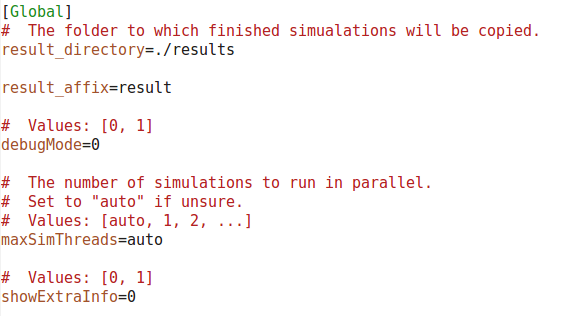
\includegraphics[width=0.6\textwidth]{config-example.png}
  \end{itemize}
\end{frame}

\begin{frame}
  \frametitle{Nebenläufigkeit}

  \begin{itemize}
  \item Probleme
    \begin{itemize}
    \item gemeinsame Dateien $\rightarrow$ ein Lauf pro Installation
    \item keine persistente Ausgabe
    \end{itemize}
  \item<2-> Lösung
    \begin{itemize}
    \item ``out of source'' Simulation (Pfad: results/)
    \item Logging dateien mit Zeitstempel.
    \end{itemize}

  \end{itemize}
\end{frame}
